\section{Linee evolutive}\label{linee-evolutive}

Il Web è la piattaforma software più estensiva al mondo, e la sua
evoluzione è stata guidata da una serie di innovazioni tecnologiche che
hanno permesso di realizzare applicazioni sempre più complesse e
performanti. Questo capitolo ripercorre brevemente le linee evolutive
del web, partendo dalle pagine statiche fino ad arrivare alle
applicazioni web moderne.

\subsection{Pagine statiche}\label{pagine-statiche}

Il primo modello del World Wide Web era orientato a facilitare la
condivisione di documenti, permettendo ai lettori di esplorarli
attraverso collegamenti tra le pagine. Il WWW consisteva in una
combinazione di applicazioni, di protocolli e di linguaggi di marcatura
progettati e rilasciati presso il CERN, principalmente ad opera di Tim
Berners Lee e Robert Calliau, a ridosso degli anni '90:

\textbf{Browser e Server:} Con un browser web installato nel proprio
sistema informatico, un utente può visualizzare pagine web e scegliere
di seguire i collegamenti ipertestuali per accedere ad altre pagine. Il
server web è responsabile di fornire le pagine web richieste dai client,
come i browser.

\textbf{Protocollo HTTP:} È il protocollo di comunicazione di livello
applicativo (OSI 7) che permette la trasmissione di informazioni tra
client e server web. Un browser contatta un server web inviando una
richiesta HTTP ad un determinato URL e il server risponde con una
risposta HTTP contenente i dati richiesti. HTTP è un protocollo
stateless, non mantiene informazioni sullo stato della comunicazione.
Sta all'applicazione gestire eventuali sessioni o autenticazioni.

\textbf{Linguaggio HTML:} (HyperText Markup Language) è un linguaggio di
marcatura utilizzato per la realizzazione di pagine web. HTML definisce
la struttura e il contenuto di una pagina web attraverso l'uso di tag e
attributi e consente di incorporare elementi multimediali. Il browser
web interpreta il codice HTML e mostra la pagina web all'utente, con una
resa grafica determinata da alcune regole.

Nel 1993, il primo browser web grafico, Mosaic, sviluppato da Marc
Andreessen e Eric Bina, introdusse il supporto per le immagini e per i
collegamenti ipertestuali, e successivamente Netscape Navigator 1.0,
sviluppato da Netscape Communications Corporation, introdusse il
supporto per CSS, il linguaggio che definisce le regole di presentazione
di una pagina. Queste innovazioni contribuirono a rendere il web più
accessibile e visivamente attraente.

\subsection{Pagine dinamiche}\label{pagine-dinamiche}

I primi browser web erano in grado di visualizzare solo pagine statiche,
il che significa che il contenuto di una determinata pagina non cambiava
in base all'interazione dell'utente\footnote{Le uniche interazioni che
  avevano effetto immediato nella pagina erano quelle di CSS, come il
  cambio di colore di un link al passaggio del mouse.}, ed i primi
server web erano in grado di fornire solo pagine statiche, cioè pagine
il cui contenuto non cambiava in maniera automatizzata.

Tramite hyperlinks e successivamente tramite form (cioè dei moduli
compilabili con opzioni, introdotte nel 1993) i browser potevano
effettuare richieste al server inviando parametri tramite il protocollo
HTTP. Il server poteva elaborare tali richieste e restituire una
\emph{nuova pagina HTML} in base ai parametri ricevuti. Questo processo
era gestito da programmi detti \textbf{CGI} (Common Gateway Interface),
da eseguire sul server per generare pagine dinamicamente, cioè al
momento della richiesta.

I linguaggi di programmazione utilizzati all'epoca per scrivere
programmi CGI erano principalmente:

\subparagraph{Linguaggi di basso livello o di
scripting}\label{linguaggi-di-basso-livello-o-di-scripting}

\begin{itemize}
\item
  Linaguaggi di basso livello come C o C++, erano di difficile gestione
  e manutenzione: sono performanti ma richiedono molte risorse per la
  progettazione.
\item
  Linguaggi di scripting come Perl o Shell UNIX, erano più facili da
  utilizzare ma meno efficienti: comodi per la manipolazione di stringhe
  e file, ma non per la gestione di strutture dati complesse.
\end{itemize}

\subparagraph{Linguaggi di templating}\label{linguaggi-di-templating}

Successivamente, dal 1995 in poi, emersero alcuni Linguaggi di
templating che consentono di incorporare codice dinamico all'interno di
pagine HTML dal lato server.

\begin{itemize}
\item
  Java Server Pages (JSP) è un'estensione di Java, quindi era possibile
  usare tutte le librerie di questo linguaggio molto popolare all'epoca.
\item
  PHP è un linguaggio interpretato che ha avuto molto successo per oltre
  un decennio\footnote{\href{https://www.tiobe.com/tiobe-index/php/}{Indice
    TIOBE per PHP}, si può vedere come il suo utilizzo sia diminuito a
    partire dal 2010.} grazie alla sua semplicità.
\end{itemize}

\begin{minted}[]{php}
<?php
$username = $_POST["username"];
$password = $_POST["password"];

$query = sprintf( "SELECT * FROM Users WHERE username='%s' AND password='%s'",
    $username, $password);
$result = mysql_query($query, $conn);

if (mysql_num_rows($result) > 0){
?>
    <h1>Benvenuto <?php echo $username; ?></h1>
    ...
<?php
    } else {
    ?>
        <h1>Accesso negato</h1>
        <p>Torna alla <a href="login">pagina di login</a></p>
    <?php
    }
?>
\end{minted}

\begin{quote}
Un esempio di pagina di autenticazione in PHP, che riflette lo stile di
programmazione tipico dell'epoca\footnote{La libreria mysql di Micheal
  Widenius per PHP 2 risale al 1996.}. È da notare come il codice HTML
da inviare al browser sia inserito direttamente all'interno del codice
da mantenere privato nel lato server, rendendone difficile la
manutenzione per via della \emph{confusione tra logica di presentazione
e logica di business}. Vengono poi adoperati 3 linguaggi diversi (PHP,
HTML, SQL), soluzione non ottimale per la leggibilità, che si aggiunge
ai problemi di sicurezza legati all'\emph{interpolazione} di stringhe
all'interno di query SQL.
\end{quote}

\subsection{Pagine attive con
Javascript}\label{pagine-attive-con-javascript}

Il dinamismo delle pagine web supportato da server CGI e linguaggi di
scripting era comunque limitato per via del caricamento di nuove pagine
ad ogni richiesta. Non era possibile aggiornare parzialmente la pagina,
ma solo scaricarne una nuova. Nel 1995 il Netscape Navigator 2.0
introdusse il supporto ad un nuovo linguaggio di scripting, che
successivamente venne chiamato Javascript, realizzato da Brendan Eich,
per ovviare a questo problema.

\begin{figure}
\centering
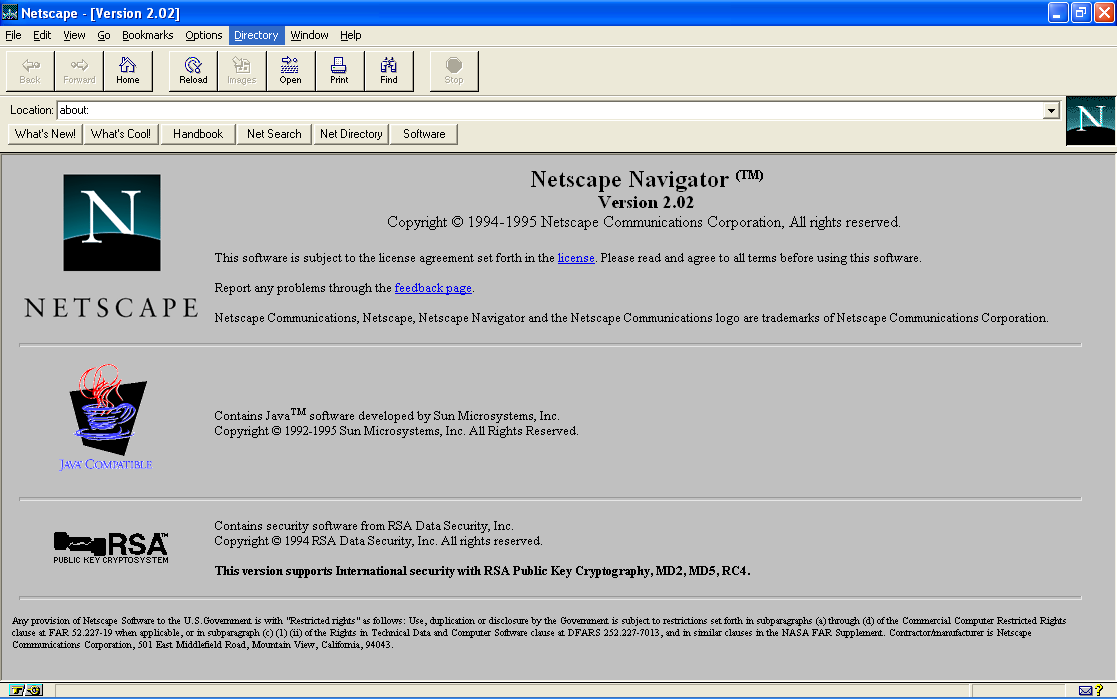
\includegraphics[width=\textwidth,height=1cm]{./res/netscape_navigator.png}
\caption{Screenshot di Netscape Navigator 2.0}
\end{figure}

\textbf{Gestione di eventi e manipolazione del DOM:} Uno script
Javascript, distribuito all'interno di una pagina HTML, può essere
eseguito dal browser web in risposta a determinati eventi dell'utente.
Inizialmente il motore di esecuzione era sincrono, cioè bloccava
l'esecuzione del codice fino al completamento dell'operazione, e le
possibilità di javascript si limitavano alla manipolazione a
\emph{runtime}\footnote{Il momento in cui la pagina è resa attiva con
  Javascript.} del DOM (Document Object Model), quindi ad aggiungere,
rimuovere o modificare elementi HTML.

\textbf{Richieste HTTP asincrone:} Le pagine web, erano diventate
\emph{attive}, ma tutte le risorse da fornire agli utenti dovevano
essere inserite nella pagina inviata come prima risposta HTTP. Nel 1999
però, il browser Internet Explorer 5 introdusse una estensione del
linguaggio Javascript, che disponeva di un oggetto chiamato
\emph{XMLHttpRequest}, in grado effettuare richieste HTTP asincrone al
server e dunque ricevere risposte senza dover ricaricare l'intera
pagina. Così si gettavano le basi per la realizzazione di \emph{Single
Page Applications}.

La libreria jQuery, rilasciata nel 2006, ha rivestito una particolare
importanza perché semplificava la manipolazione del DOM e le richieste
HTTP, fornendo un'interfaccia più semplice e omogenea rispetto ai
diversi browser, che esponevano API diverse e non ancora standardizzate.

\begin{minted}[]{javascript}
$('#update').click(function() {
    $.ajax({ // scaricamento asincrono
        url: 'data.json', type: 'GET', dataType: 'json',
        success: function(data) {
            var content = '';
            for (var i = 0; i < data.length; i++) {
                content += '<p>' + data[i].name + '</p>';
            }
            $('#content').html(content);
        },
    });
});
\end{minted}

\begin{quote}
Nel frammento di codice jQuery, è messo in evidenza uno stile
\emph{imperativo} di definizione del comportamento dell'interfaccia,
poco manutenibile per applicazioni complesse.
\end{quote}

\subsection{Node.js e Javascript lato
server}\label{node.js-e-javascript-lato-server}

La standardizzazione di Javascript procedette attraverso le varie
versioni di ECMAScript che definivano le nuove funzionalità del
linguaggio e, di conseguenza, dei browser web. Nel 2008 fu rilasciata la
prima versione di Google Chrome, un browser che, oltre ad includere
caratteristiche appetibili per gli utenti finali, disponeva del motore
di esecuzione Javascript V8. Questo \emph{engine} apportò dei
sostanziali miglioramenti di prestazioni\footnote{\href{https://youtu.be/LRmrMiOWdfc?si=gaHRFdA8QcYZ0NYq&t=2676}{Google
  Chrome announcement:} in questo video si può vedere come l'esecuzione
  di Javascript su Chrome sia di circa 60 volte più veloce che su
  Internet Explorer 8.} rispetto alla competizione e venne rilasciato
come \emph{Open source software}.

Nel 2009, Ryan Dahl iniziò a lavorare, basandosi sul codice di V8, a
Node.js, un interprete di Javascript in modalità headless\footnote{Cioè
  senza interfaccia grafica.}, al quale aggiunse la capacità di accedere
al filesystem, di esporre servizi HTTP e di accettare connessioni in
maniera \emph{non bloccante}.

In questo modo si poterono realizzare non solo applicazioni
\textbf{frontend} ma anche \textbf{backend} con Javascript, abilitando
sempre più novizi alla creazione di siti web completi. Attorno a Node
crebbe una comunità di sviluppatori che contribuirono, secondo i
principi dell'Open source, alla creazione di un ecosistema di librerie,
che potevano essere installate tramite il gestore di pacchetti NPM.

\begin{minted}[]{javascript}
const http = require("http");
const mysql = require("mysql");

const connection = mysql.createConnection({ /* ... */ })

const server = http.createServer((req, res) => {
    if (req.method === 'POST' && req.url === '/login') {
        var username, password;
        // unmarshalling della query string ...
        var login = "SELECT * FROM Users WHERE username = ? AND password = ?";
        connection.query(login, [username, password], (err, rows) => {
            if (rows.length > 0) {
                res.writeHead(200, {"Content-Type": "text/html"});
                res.end("<h1>Benvenuto " + username + "</h1>");
            } else {
                res.writeHead(401, {"Content-Type": "text/html"});
                res.end("<h1>Accesso negato</h1>");
            }
        });
    }
});
server.listen(80, () => { console.log("Server in ascolto alla porta 8080"); });
\end{minted}

\begin{quote}
In questo frammento di codice è mostrato l'utilizzo della libreria
``http'' fornita di default da Node e della libreria ``mysql'' di Felix
Geisendörfer, una delle prime per l'accesso a database da Node. È da
notare l'architettura a callback, che permette di gestire in maniera
asincrona le richieste HTTP e le query al database.
\end{quote}

\begin{quote}
In questo esempio le query SQL sono parametrizzate, facendo uso di
\emph{Prepared statements}, per evitare attacchi di tipo injection, ma
rimangono cablate all'interno di stringhe, rendendo il codice
vulnerabile a errori di sintassi e di tipo.
\end{quote}

\subsection{Applicazioni web orientate a
componenti}\label{applicazioni-web-orientate-a-componenti}

Anche con Node fu possibile realizzare applicazioni web
\emph{monolitiche}, parimenti al templating PHP, usando librerie come
EJS di TJ Holowaychuk.

Tuttavia le tendenze di quel periodo (circa 2010) si discostarono dal
modo tradizionale di scrivere applicazioni web, basate su pagine
generate lato server, per passare a un modello di \textbf{client-side
rendering}. Secondo questo modello il server invia al browser una pagina
HTML con un DOM minimo, corredato di script JS che si occupano di
popolare il DOM dei contenuti e di gestire le logiche di presentazione.

Le applicazioni renderizzate lato cliente potevano beneficiare di una
maggiore \emph{reattività} e di una migliore esperienza utente, essendo
basate su una pagina unica che veniva aggiornata in maniera
incrementale, aggirando i caricamenti di nuove pagine da richiedere al
server. Le richieste, essendo asincrone, potevano essere gestite in modo
meno invasivo rispetto a prima: mentre la comunicazione client-server
avveniva in background, l'utente poteva continuare ad interagire con
l'applicazione.

Il vantaggio di questo paradigma da parte degli sviluppatori era la
possibilità di scrivere la logica di presentazione interamente in
Javascript, sfruttando il sistema di oggetti e la modularità del
linguaggio in maniera più espressiva rispetto al templating o alle API
DOM.

L'idea centrale delle nuove tendenze \emph{CSR} era quella di progettare
l'interfaccia utente partendo da parti più piccole, chiamate
\textbf{componenti}, e riutilizzabili all'interno dell'intera
applicazione. Lo stile assunto era \emph{dichiarativo}\footnote{In
  questo contesto, uno stile dichiarativo è riferito ad un approccio
  alla programmazione in cui si descrive cosa il programma deve fare
  piuttosto che come farlo. Con jQuery si dovevano specificare
  esplicitamente i passaggi per manipolare il DOM, mentre i componenti
  permettono di definire il comportamento dell'interfaccia attraverso
  delle dichiarazioni più astratte e concise.}. Ad ogni componente sono
associati:

\begin{itemize}
\tightlist
\item
  un template HTML, più piccolo e gestibile rispetto ad una pagina
  intera.
\item
  un foglio CSS, per la stilizzazione.
\item
  il codice Javascript che ne definisce la logica di interazione.
\end{itemize}

Tra gli esempi più noti di sistemi di componenti:

\subparagraph{Angular.js}\label{angular.js}

Uno dei primi framework a proporre un modello di componenti, sviluppato
in Google e rilasciato nel 2010. Angular.js introduceva il concetto di
\emph{Two-way data binding}, cioè la possibilità di sincronizzare
automaticamente i dati tra il modello e la vista.

\subparagraph{React.js}\label{react.js}

La libreria di componenti più diffusa\footnote{\href{https://github.com/facebook/react}{Github
  - React} - la più popolare in base numero di stelle su Github.}
sviluppata da un team interno di Facebook e rilasciata nel 2013. React
introduceva il concetto di \emph{Virtual DOM}, una rappresentazione in
memoria del DOM reale, che permetteva di calcolare in maniera efficiente
le differenze tra due stati del DOM e di applicare solo le modifiche
necessarie.

\subparagraph{Vue.js}\label{vue.js}

Partito come progetto personale di Evan You e rilasciato nel 2014, Vue
si proponeva come un'alternativa più flessibile e meno verbosa rispetto
ad Angular e React, dai quali riprende il binding bidirezionale e il
Virtual DOM. È la libreria di componenti usata da Nuxt.

\begin{minted}[]{html}
<script setup>
    import { RouterView } from "vue-router";
    import HelloWorld from "./components/HelloWorld.vue";
</script>

<template>
    <HelloWorld msg="Ciao mondo" />

    <RouterView />
</template>

<style scoped>
    background-color: #f0f0f0;
</style>
\end{minted}

\begin{quote}
Un esempio moderno di applicazione Vue 3, che mostra l'utilizzo di un
componente ``HelloWorld'' all'interno di un template principale, e di un
RouterView per la navigazione tra le pagine. Questi componenti sono
definiti in file distinti, per favorire la separazione delle
preoccupazioni, ed importati nel file principale come se fossero moduli
Javascript. Ogni volta che compaiono in un template assumono un
comportamento dettato dalla loro definizione (il loro template) e dal
loro \emph{stato} di istanza. Si noti come il componente HelloWorld sia
parametrizzato con un attributo ``msg'', che ne consente un utilizzo più
flessibile.
\end{quote}

\begin{minted}[]{html}
<html lang="en">
    <head>
        <title>Vite App</title>
    </head>
    <body>
        <div id="app"></div>
        <script type="module" src="/src/main.js"></script>
    </body>
</html>
\end{minted}

\begin{quote}
Il DOM minimo che viene distribuito da una applicazione Vue 3. La pagina
viene assemblata lato client, a partire dal così detto \emph{entry
point}: l'elemento con id ``app'', in cui viene montata l'applicazione.
Si noti che nel caso che Javascript non sia abilitato nel client il
contenuto dell'applicazione non verrà visualizzato affatto.
\end{quote}

\subsection{Typescript e ORM}\label{typescript-e-orm}

Le basi di codice Javascript iniziarono a diventare sempre più complesse
quando anche i team di sviluppatori di grandi compagnie iniziarono ad
adottare i framework a componenti. A partire dal 2014 anche applicazioni
web come Instagram, Netflix e Airbnb incorporarono React nei loro stack
tecnologici per realizzare interamente l'interfaccia utente.

Javascript, essendo un linguaggio interpretato e debolmente tipizzato,
non era in grado di garantire la correttezza del codice e i test di
unità erano fatti in modo \emph{behavior driven}, cioè basati sul
comportamento dell'applicazione e non sulla tipizzazione dei dati.
Questo spesse volte portava ad errori, difficili da individuare e
correggere, soprattutto in applicazioni di grandi dimensioni.

Nel 2012 Anders Hejlsberg ed il suo team interno a Microsoft iniziarono
a lavorare al linguaggio Typescript, una estensione di Javascript,
realizzando un \textbf{compilatore} in grado di rilevare errori di tipo
in con analisi statica. Typescript permette anche di sfruttare le
funzionalità delle nuove versioni di ECMAScript in modo
\emph{retrocompatibile}, cioè facendo \emph{transpiling}\footnote{\href{https://en.wikipedia.org/wiki/Source-to-source_compiler}{Wikipedia
  - Source-to-source compiler} - il transpiling è il processo di
  traduzione automatica di codice sorgente da un linguaggio ad un altro.}
verso una specifica di ECMA inferiore, per usarle anche sui browser
deprecati.

L'adozione di Typescript è stata pressoché immediata, per il motivo che
la conversione di basi di codice a partire da Javascript
vanilla\footnote{Con ``vanilla'' ci riferisce a Javascript senza
  estensioni, quindi al codice che può eseguire nativamente sui browser
  conformi alle specifiche ECMA. Typescript invece è un \emph{superset},
  quindi ha un insieme di espressioni sintattiche più grande ma che
  comprende interamente quello di Javascript.} era a costo zero: ogni
sorgente Javascript è valido Typescript. Typescript ha avuto successo
non solo lato client, ma anche lato server. Sono comparse infatti alcune
librerie di supporto all'accesso a database basate sul pattern
\textbf{ORM}, \emph{Object-relational mapping}, quindi capaci di mappare
il modello dei dati presente nel database a strutture dati proprie di
Typescript. Librerie notevoli di questo tipo sono:

\subparagraph{Sequelize}\label{sequelize}

È stata una delle prime, il progetto è iniziato nel 2010 quindi
funzionava con Javascript vanilla, ma si è evoluta fino a supportare le
migliorie di Typescript ed una moltitudine di DBMS.

\subparagraph{TypeORM}\label{typeorm}

Offre un supporto a Typescript nativamente. È illustrata con dettaglio
nel \hyperref[descrizione-delle-tecnologie]{capitolo 2}.

\subsection{Ritorno al server side
rendering}\label{ritorno-al-server-side-rendering}

Dal lancio di React sempre più applicazioni web hanno fatto uso della
tecnica CSR per via della migliorata esperienza utente e di sviluppo.
Questo approccio ha portato però una serie di nuovi problemi e
limitazioni legate al meccanismo di rendering.

\subparagraph{Performance su dispositivi
lenti}\label{performance-su-dispositivi-lenti}

I \emph{bundle} Javascript che vengono generati per le applicazioni CSR
sono spesso onerosi in termini di risorse, e la loro esecuzione su
dispositivi con capacità di calcolo limitate può risultare lenta e
insoddisfacente per l'utente.

\subparagraph{Search engine
optimization}\label{search-engine-optimization}

I siti web che fanno uso di CSR sono più difficilmente indicizzabili dai
\emph{crawler} dei motori di ricerca, questo può portare a problemi di
esposizione e di traffico ridotti.

\subparagraph{First contentful paint}\label{first-contentful-paint}

È il tempo che intercorre tra la cattura della risposta HTTP del server
e il momento in cui viene visualizzato a schermo dal browser il primo
elemento di contenuto significativo per l'utente. Nelle applicazioni CSR
questa durata spesso eccede quella massima suggerita da
Google\footnote{\href{https://developers.google.com/search/docs/appearance/core-web-vitals?hl=it}{Google
  developers - Core web vitals} - Al 10 maggio 2023, la durata massima
  ammissibile per il FCP è di 2.5s.}.

\subparagraph{Cumulative shift layout}\label{cumulative-shift-layout}

Per il motivo che gli aggiornamenti dell'interfaccia vengono vengono
resi graficamente nel browser in maniera sequenziale, potrebbero esserci
dei fastidiosi spostamenti di elementi visivi nell'interfaccia.

\subparagraph{Accessibility}\label{accessibility}

Per gli stessi motivi che portano a CSL, ci potrebbero essere degli
impedimenti di accessibilità per chi usa metodi di input alternativi o
per gli screen-reader che aiutano le persone non vedenti nella fruizione
delle pagine web.

\begin{center}\rule{0.5\linewidth}{0.5pt}\end{center}

Per questi motivi, a partire dal 2016, sono emerse delle nuove tendenze
che hanno portato ad un ritorno al server side rendering, in
combinazione con i sistemi basati su componenti, per unire i vantaggi di
entrambi i modelli. Esempi di framework che supportano il SSR sono:
Angular Universal, Next.js per React e Nuxt per Vue, che verrà
illustrato nel \hyperref[descrizione-delle-tecnologie]{capitolo 2}, per
la realizzazione di applicazioni web \emph{fullstack}\footnote{Si
  occupano sia di frontend che di backend.}.
